% !TeX root = ../pythonTutorial.tex
\chapter{Grundlagen}

\section{Was ist Python?} %TODO ADD INFORMATION AND INTRODUCTION
\label{grundlagen:sec:WasIstPython}
Die Programmiersprache Python wurde Anfang der 1990er Jahre von Guido van Rossum entwickelt.
Der Name der Sprache beruht auf der Komikergruppe  Monty Python.
Hierzu lassen sich auch zahlreiche Anspielung in der Dokumentation von Python finden.
Python wurde mit dem Ziel gr��ter Einfachheit sowie �bersichtlichkeit entworfen.
Dies wird nicht zuletzt durch die Gr��e �bersichtlichkeit in der Standardbibliothek versucht zu erreichen sondern auch durch die Modulare Erweiterbarkeit.
Im Folgenden wird die Programmiersprache Python in der Version 3 behandelt.

\section{Installation}
\randnotiz{Installation}
\label{grundlagen:sec:Installtion}
Python kann auf der Webseite \url{https://www.python.org} f�r eine Vielzahl von Betriebssystemen bezogen werden. 
Es stehen 32- und 64-Bit Versionen zur Verf�gung. 
Nach dem Start des Installationsassistenten f�hrt er den Nutzer durch den Installationsprozess. 
Der Ablauf der Installation unterscheidet sich zwischen den Betriebssystemen nur gering bis gar nicht.
Nach erfolgreichem Abschluss stehen dem Anwender verschiedene Programme und zur Arbeit mit Python zur Verf�gung.
Im vom Nutzer gew�hlten Installationsverzeichnis befinden sich nun folgende Programme: 
\begin{description}
    \item[\textit{IDLE}] Standard IDE\footnote{Integrated Development Environment} f�r Python
    \item[Python] Standard Konsolen Interpreter
    \item[Pythonw] Standard Interpreter ohne Konsolenausgabe
\end{description}
Diese Programme reichen aus, um Code mit Python zu entwickeln. 
Der Python Interpreter kann nun in der Konsole mit dem Befehl ''python'' aufgerufen werden. 
Die folgenden Abschnitte beschreiben Besonderheiten bei der Installation auf einzelnen Betriebssystemen. 
\subsection{Hinweis zur Installation unter Windows}
\label{grundlagen:sec:InstallationWindows}
Windows Nutzer m�ssen die Systemvariable f�r Python im Installationsassistenten hinzuf�gen lassen. 
Andernfalls kann Python nur im Installationsverzeichnis bzw. durch die Angabe des kompletten Pfades aufgerufen werden. 
In Abbildung \ref{grundlagen:img:InstallationWindows} ist die notwendige Auswahl zu sehen. 
\begin{figure}[ht]
\centering
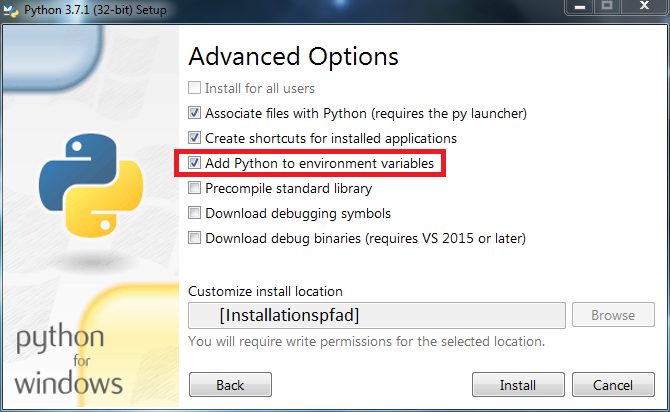
\includegraphics[scale=0.5]{images/InstallationWindows.png}
\caption{Start des Installationsassistenten}
\label{grundlagen:img:InstallationWindows}
\end{figure}
%
\subsection{Hinweis zur Installation unter Mac}
\label{grundlagen:sec:InstallationMac}
Im Folgenden wird die Installation unter macOS X gezeigt.

\begin{figure}[ht]
	\centering
	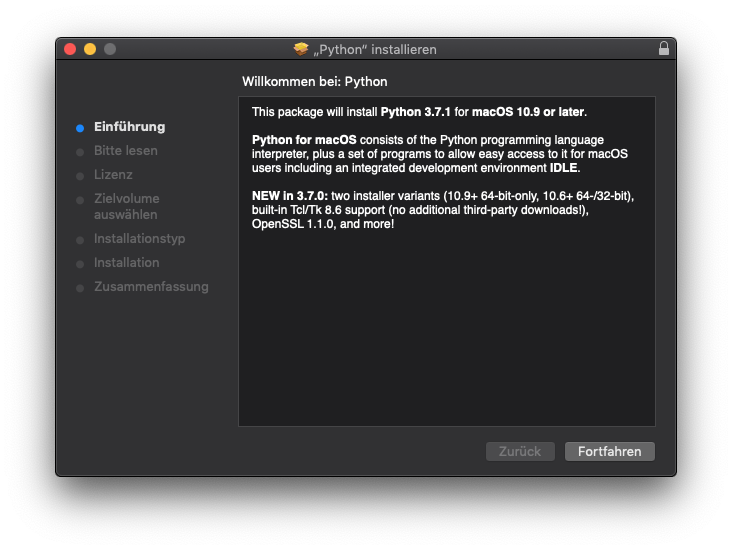
\includegraphics[scale=0.5]{images/InstallationMac.png} 
	\caption{Start des Installationsassistenten}
	\label{grundlagen:img:InstallationMac}
\end{figure}
Nach Ende der Installation befindet sich der Python Ordner im Finder (Dateiexplorer).

\begin{figure}[ht]
	\centering
	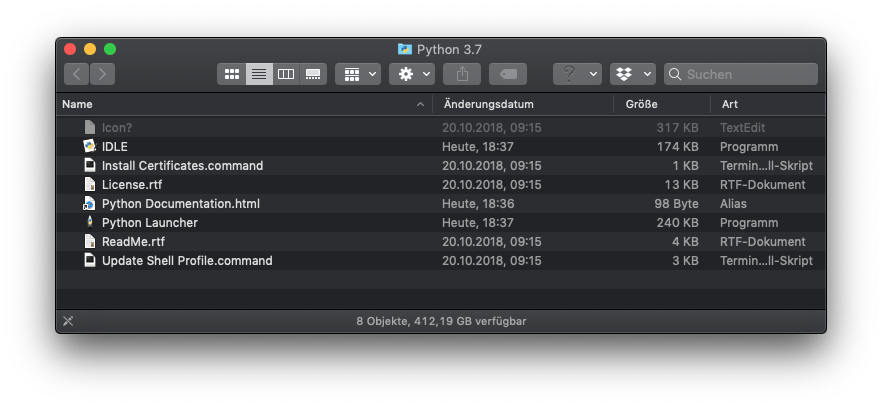
\includegraphics[scale=0.5]{images/PythonFinder.png} 
	\caption{Fertige Installation}
	\label{grundlagen:img:FinishInstall}
\end{figure}
Zuletzt wurde durch den Assistent unter /Library/Frameworks/Python.framework noch das Python Framework abgelegt.
Ohne dieses w�re das Arbeiten mit Python unter Mac nicht m�glich.

\subsection{Hinweis zur Installation unter Linux(Ubuntu)}
\label{grundlagen:sec:InstallationLinux}
Im Folgenden wird die Installation f�r Ubuntu Version 18.04.1 LTS erl�utert.
Im Gegensatz zu den anderen Betriebssystemen, wird hier von Haus aus ein Python Interpreter in der Version 3.6.6 mitgeliefert, jedoch nicht die Standard Entwicklungsumgebung IDLE.
Diese kann �ber das Paket \textit{IDLE} nachtr�glich installiert werden.
Sollte trotzdem noch kein Python vorhanden sein, durch den folgenden Befehl die Installation manuell angesto�en werden.

\begin{lstlisting}[language=BASH, label={grundlagen:lst:InstallationLinux}]
sudo apt-get install python3 python-doc
\end{lstlisting}

Diese Installation umfasst unter anderem auch die Dokumentation von Python.
Nach Abschluss der Installationsroutine kann wie mit jedem anderen Betriebssystem mit Python gearbeitet werden.

%TODO Skript versus Programm
\section{Python Interpreter} %WIP ROGU 
\label{grundlagen:sec:Interpreter}
%TODO ADD LINKS TO OTHER SECTIONS %WHAT IS PYTHON CODE?
Die einfachste M�glichkeit, Python Code auszuf�hren, ist direkte �bergabe des Codes an den sogenannten Python Interpreter. 
Dabei handelt es sich um eine Konsolenanwendung, welche Code ausf�hren und gegebenenfalls auftretende Ergebnisse ausgeben kann. 
Dabei kann ein Nutzer den Code entweder direkt in die Konsole eingeben oder diesen aus einer Datei auslesen lassen. 
Wie bei anderen Programmiersprachen auch, stehen f�r Python verschiedene IDEs zur Verf�gung, welche in Kapitel \ref{} behandelt werden. 
F�r die ersten Versuche mit Python reicht der Interpreter jedoch v�llig aus. Dieser wird standardm��ig mit Python installiert.

In Abbildung \ref{grundlagen:img:Interpreter} ist der Interpreter zu sehen. 
Zus�tzlich zur Version werden auch noch der Herausgeber von Python, sowie die Uhrzeit angezeigt.
Bereits jetzt kann erster Code ausgef�hrt werden.
Im Folgenden werden zu einzelnen Bestandteilen von Python Beispiele beigef�gt, welche leicht im Interpreter ausf�hrbar sind. Es wird dem Leser empfohlen, diese zum besseren Verst�ndnis nachzuvollziehen, falls m�glich durch eigenst�ndiges Ausprobieren.

\begin{figure}[ht]
	\centering
	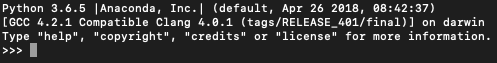
\includegraphics[width=0.8\textwidth]{images/Interpreter.png} 
	\caption{Ansicht nach Start des Interpreters}
	\label{grundlagen:img:Interpreter}
\end{figure}
 
\subsection*{Interaktiver Modus} 
\label{grundlagen:sec:InteraktiverModus}
Wird der Interpreter ohne Angabe einer Quellcodedatei gestartet, befindet dieser sich im interaktiven Modus. 
Der Nutzer kann hier direkt Anweisungen eingeben. Durch die Ausgabe der Zeichen $>>>$ zeigt die Konsole an, dass sie eine Anweisung erwartet. 
In Python existieren auch mehrzeilige Anweisungen. 
Nach der Eingabe der ersten Zeile, werden die Zeichen $...$ ausgegeben, was bedeutet, dass Folgeanweisungen erwartet werden. 
\subsection*{Einlesen einer Datei} %WIP ROGU
\label{grundlagen:sec:EinlesenDatei}
Dateien, welche Python Code enthalten werden mit der Dateiendung ''.py'' gekennzeichnet. 
Sie k�nnen direkt mit dem der Konsole ausgef�hrt werden.
Dazu muss der ausf�hrbaren Datei ''python.exe'' der Pfad der Python-Datei �bergeben werden.
\section{Syntax}
\label{grundlagen:sec:Syntax}
Im Folgenden werden wichtige Grundkonzepte der Sprache Python erl�utert.
%\subsection{Ausdr�cke} %WIP ROGU
%Anders als bei anderen Programmiersprachen wie beispielsweise Java, ben�tigt Python keine Klassenkonstrukte... %TODO AUSDRÜCKE, kein fester Rahmen zur Ausführung benötigt
%\subsection{Einfache Datentypen}
%TODO REMOVE SUBSECTION
\subsection{Leerzeichen und Einr�ckung} %TODO FORMULIERUNG
\label{grundlagen:sec:LeerzeichenEinrueckung}
Um in Python Bl�cke auszuzeichnen werden im Gegensatz zu Java oder C++ keine geschweiften Klammern genutzt.
In Python werden Bl�cke durch das Einr�cken der Zeilen markiert.
In Python ist hierf�r entweder der Tabulator oder 4 aufeinander folgende Leerzeichen vorgesehen.
%Somit kann bei zum Beispiel einer IF-Abfrage der nachfolgende Block leicht falsch zugeordnet werden wenn in den nachfolgenden Zeilen die Einr�ckung �bersehen wird.
%TODO REMOVE? if abfragen sind noch nicht eingef�hrt worden
\subsection{Kommentare}
\label{grundlagen:sec:Kommentare}
Innerhalb der Programmiersprache Python wird zwischen Zeilen- und Blockkommentaren unterschieden.
Zeilenweise Kommentare werden durch das Rautensymbol (\# ) eingeleitet.
Blockkommentare hingegen werden durch drei aufeinander folgende Anf�hrungszeichen  $''''''$ jeweils zu Beginn und am Ende des Kommentares markiert.
Hier wird jeweils ein Beispiel gezeigt:

\lstinputlisting[language=Python,label={grundlagen:lst:Kommentare}]{chapters/basics/src/comment.py}
\subsection{Typsicherheit}
\label{grundlagen:sec:Typsicherheit}
Anders als bei Java und C++ ist Python eine nur schwach typisierte Sprache.
Somit ist bei der Initialisierung keine Typangabe erforderlich.
Der Datentyp wird beim Initialisieren dynamisch ermittelt und automatisch zugewiesen.
Um einer Variable trotzdem einen gew�nschten Typ zuzuweisen, kann man sie einfach mit dem entsprechenden Typ initialisieren.
Weitere Informationen zu Datentypen werden in Abschnitt \ref{} erl�utert. %TODO ADD REF


%\subsection{Prozedurale Programmierung} %TODO NOT NEEDED ANYMORE?

\section{Beispiel \glqq Hello World!\grqq} %TODO ADD MORE STUFF
\randnotiz{Beispiel}
\label{grundlagen:sec:HalloWorld}
Einfache Ausgaben k�nnen mit dem print()- Befehl ausgef�hrt werden. 
Innerhalb der Klammern muss ein String �bergeben werden, eine einfache Zeichenkette. 
Diese wird durch umschlie�ende einfache oder doppelte Anf�hrungszeichen markiert (''EinString''/'EinString'). 
Der Einfachheit halber, wird hier noch auf die genaue Erkl�rung der einzelnen Bestandteile der Anweisung verzichtet. 
Mehr erf�hrt der Leser in sp�teren Kapiteln. Ein einfaches ''Hello-World!''-Programm ben�tigt in Python tats�chlich nur eine Zeile: 

\lstinputlisting[language=python, label={grundlagen:lst:HalloWorld}]{chapters/basics/src/helloworld.py}
Es handelt sich dabei um ein vollst�ndiges Python-Programm, welches in dieser Form ausgef�hrt werden kann. 
Anders als bei Java oder C++ werden keinerlei Klassenkonstrukte oder main-Methoden ben�tigt.
\section{�bung}
\randnotiz{�bung}
\label{grundlagen:sec:Uebung}
Im folgenden sollen die zuvor gelernten beziehungsweise gezeigten Punkte anhand von �bungen wiederholt und vertieft werden.
\uebung
\aufgabe{grundlagen01} 
\aufgabe{grundlagen02}
\section{Zusammenfassung} %TODO MOVE TO END OF THE CHAPTER
\label{grundlagen:sec:Zusammenfassung}
In diesem Kapitel hat der Leser seine ersten Schritte mit der Sprache Python gemacht. 
Es wurde grundlegend vorgestellt, wobei es sich bei Python �berhaupt handelt und wie die Programmiersprache installiert wird. 
Es wurde der Python Interpreter vorgestellt, einer einfachen Konsolenanwendung zur Ausf�hrung von Python Code. 
Weiterhin wurden Kommentare und die Blockstruktur eingef�hrt. 
Um das in diesem Kapitel erlangte Wissen anzuwenden, wurde ein klassisches Hello-World! Programm geschrieben. 
Die Inhalte dieses Kapitels, vor allem die Installation, sollten vom Leser verstanden worden sein, bevor er mit dem Rest des Tutorials  fortf�hrt.


% !TeX root = ../../pythonTutorial.tex
\section{IDEs}\label{ides:section:ides}

Python Programmierung mit der IDLE (in Python integrierte Entwicklungsumgebung) oder Python Shell sind gute\randnotiz{IDLE}
M�glichkeiten um den Einstieg in Python  zu vereinfachen. 
Ein grunds�tzliches Verst�ndnis der Sprache und erste kleine Programme lassen sich so bew�ltigen. 
Sobald jedoch gr��ere Programme oder Projekte anstehen kann es mit diesen Tools schnell frustrierend werden.

Eine passende IDE (Integrierte Entwicklungsumgebung) oder selbst ein einfacher Code-Editor kann einem das leben deutlich vereinfachen. Im folgenden werden einige geeigneten IDEs f�r Python vorgestellt und f�r jede einige Vor- und Nachteile aufgezeigt.

\subsection*{Was ist eine IDE?}
Integrierte Entwicklungsumgebungen vereinen wichtige Tools f�r das Erstellen von Software unter einer Oberfl�che. Dazu z�hlen Editor mit Syntax-Hervorhebung, Compiler, Debugger, Interpreter und weitere Werkzeuge, die dem Entwickler die Arbeit erleichtern.

Durch den Austausch zwischen Werkzeugen innerhalb der IDE k�nnen Arbeitsg�nge erleichtert und beschleunigt werden. Fehler im Quelltext beispielsweise k�nnen direkt in der entsprechenden Zeile markiert werden.

\subsection*{Anforderungen an eine Python Entwicklungsumgebung}
Es gibt ein paar Grundanforderungen an eine geeignete oder gute Python Entwicklungsumgebung:

\begin{description}
\item[Debugging Unterst�tzung]\hfill \\
Schrittweise durch den Code zu wandern, w�hrend dieser ausgef�hrt wird, ist eine weiter Grundaufgabe einer IDE.
\item[Syntax Highlighting]\hfill \\
Farbliche Markierungen erleichtern die Suche nach bestimmten Keywords. Die Lesbarkeit des Codes wird hierdurch verbessert.
\item[Automatische Codeformatierung]\hfill \\
Eine gute IDE erkennt das Zeilenende beispielsweise nach einem \textit{While-Statement} und r�ckt die n�chste Zeile automatisch ein.
\item[Ausf�hren des Codes innerhalb der IDE]\hfill \\
Wenn der Code au�erhalb der IDE ausgef�hrt werden muss, ist es eher ein Text-Editor als eine IDE.
\item[Interaktive Console]\hfill \\
Live Ein- und Ausgabe einzelner Codezeilen.
\item[Fehlererkennung]\hfill \\
Syntaxfehler sollten automatisch markiert werden und Runtime-Fehler genannt werden.
\end{description}

\subsection{Einige IDEs vorgestellt}
\subsubsection*{Eclipse}
Wer schon mit Java programmiert hat, ist wohl schon mal auf Eclipse gesto�en. Durch die Installation von PyDeth l�sst sich Eclipse gut (und kostenlos) f�r die Python-Entwicklung erweitern und bietet dabei wichtige Features, wie zum Beispiel Code Completion, Python Debugging, eine interaktive Python Konsole oder das Einbinden von Django.

\textbf{Vorteile:} 
Wenn Eclipse bereits auf dem Rechner vorhanden ist, gen�gt der Download der PyDeth Erweiterung, welche nach einem Neustart von Eclipse sofort eingebunden ist.

\textbf{Nachteile:}
Der Einstieg in die Python Programmierung f�r Eclipse-Neulinge kann in der sehr gro�en Entwicklungsumgebung Eclipse zu Schwierigkeiten f�hren.

\subsubsection*{Visual Studio}
Die IDE aus dem Hause Microsoft bietet viele eigene Erweiterungen und Entwicklungs-Features an, welche dem Entwickler eine gute Individualisierungsm�glichkeit bieten. Die Visual Studio Python Tools erm�glichen es, alle �blichen Entwicklungsm�glichkeiten bei Programmierung mit Python zu nutzen. Visual Studio ist sowohl in der Community-Version umsonst, aber auch in einem Bezahlmodell verf�gbar.

Visual Studio Community kann kostenlos �ber folgenden Link heruntergeladen werden: https://visualstudio.microsoft.com/de/vs/community/

\textbf{Nachteile:}
Der Download ausschlie�lich f�r die Python-Programmierung ist recht gro� (3-4GB). Es m�ssen sowohl das Programm an sich, als auch die Python-Erweiterung heruntergeladen werden. Visual Studio ist ausschlie�lich f�r Windows und MacOs verf�gbar. Eine Linux-Variante wird allerdings von Visual Studio Code angeboten. Vergleichbar mit Eclipse ist auch Visual Studio nicht sonderlich einsteigerfreundlich.

\subsubsection*{Atom}
Etwas schlichter geht es im Atom Editor zu. Das klare und strukturierte Interface ist auch f�r Einsteiger gut verst�ndlich und dient daher als geringere H�rde, die ein Neuling �berwinden muss, als die �berladenen Interfaces von Eclipse oder Visual Studio. Python kann durch eine Erweiterung nachtr�glich installiert werden, welche w�hrend der Laufzeit hinzugef�gt werden kann.

\textbf{Vorteile:}
Einsteigerfreundliche Alternative mit geringem Download- und Installationsumfang, sowie Plattformunabh�ngigkeit.

\textbf{Nachteile:}
\textit{Build-} und \textit{Debugging-Support} sind keine eingebauten Features, sondern nur als Community-Addon verf�gbar.


\subsubsection*{PyCharm}
PyCharm ist (wie es der Name vermuten l�sst) eine IDE explizit f�r Python. Es ist neben der Hauptdatei keine Erweiterung n�tig, ein neues Projekt kann sofort gestartet und mit dem Programmieren sofort begonnen werden. PyCharm ist Plattformunabh�ngig und sowohl in einer freien Open-Source-Version nutzbar, als auch in einer kostenpflichtigen Pro-Version erh�ltlich.

\textbf{Vorteile:}
PyCharm bietet einen vielf�ltigen Support an und eine sehr aktive Community. Egal an welcher Stelle man ein Problem hat, es wird einem mit gro�er Wahrscheinlichkeit geholfen.

\textbf{Nachteile:}
Die Ladezeiten sind vergleichbar lang und an manchen Stellen finden sich kleinere Usability-Schwachpunkte.


% !TeX root = ../../pythonTutorial.tex

\section{Elementare Datentypen}
\label{grundlagen:sec:ElementareDatentypen}

�hnlich wie bei Java und C oder C++ gibt es auch in Python Variablen. Allerdings gibt es dabei immense Unterschiede zu den anderen Programmiersprachen, weshalb sich ein genauerer Blick auf die einzelnen Datentypen in jedem Fall lohnt. Bei vielen bekannten Sprachen wird einer Variablen ein bestimmter Datentyp zugeordnet (deklariert). Der Datentyp kann darauf folgend zur Laufzeit nicht wieder ge�ndert werden, der Wert innerhalb des Datentyps allerdings schon. So lassen sich in eine Variable des Typ Integer beispielsweise keine String-Werte speichern. In Python hingegen ist dies ohne weiteres m�glich. Hier wird g�nzlich auf eine explizite Typdeklaration verzichtet. Zeigt eine Variable beispielsweise auf eine ganze Zahl, so wird diese als ein Objekt vom Typ Integer interpretiert. Allerdings ist es m�glich, diese im n�chsten Schritt einfach auf ein String-Objekt zeigen zu lassen. Dies ist in Python m�glich, weil eine Variable ein Objekt lediglich referenziert und dadurch keinem Typ zugewiesen wird.\\
Betrachten wir nun die Datentypen etwas genauer.

\subsection{Zahlenoperatoren}

Da in Python auf Typdeklaration verzichtet wird, muss dies beim Anlegen von Variablen nicht ber�cksichtigt werden. Wird eine ganze Zahl (Integer) ben�tigt, kann diese, falls n�tig, auch in eine Gleitkommazahl (float) umgewandelt werden, ohne viel am Code zu �ndern. Python deklariert im Hintergrund selbst und spart so unn�tige Komplexit�ten und Fehlerquellen. (Beispiel \ref{refzahl})

\begin{lstlisting}[label=refzahl]
# Zahlenoperatoren
i = 42
type(i)
// Ausgabe: <class 'int'>
i = 42.22
type(i)
// Ausgabe: <class 'float'>
\end{lstlisting}

\textbf{Boolean}

Boolean gibt an, ob ein Statement \textit{true} oder \textit{false} ist. Dadurch lassen sich Fallunterscheidungen oder Abfragen erm�glichen. (Beispiel in Listing \ref{basicDatatypes:lst:refbool})

\begin{lstlisting}[label=basicDatatypes:lst:refbool]
# Boolean
i = True
i
// Ausgabe: True

\end{lstlisting}

\textbf{String}

Der String ist eine Zeichenkette, also eine Aneinanderreihung von verschiedenen Zeichen. Dazu z�hlen W�rter, aber auch beispielsweise Hexadezimal-Codes oder E-Mail Adressen.

Wie in den meisten objektorientierten Programmiersprachen lassen sich auch in Python die einzelnen Zeichen eines Strings abrufen, indem der dazugeh�rige Index abgefragt wird.

Wie in Listing \ref{basicDatatypes:lst:refstring} kann die L�nge des gesamten Strings durch einfache Abfrage angezeigt werden. 

\begin{lstlisting}[label=basicDatatypes:lst:refstring]
# Strings
i = "Python"
print (i)
// Ausgabe: Python

print(i[0])
// Ausgabe: P

print(len(i))
// Ausgabe: 6

\end{lstlisting}

\subsection{ENUMs}

Enums dienen in den objektorientierten Programmiersprachen zur Aufz�hlung von Ausdr�cken einer endlichen Menge. So werden zum Beispiel Jahreszeiten, Monate oder Farben oft als Enums umgesetzt (vgl. Listing \ref{refenum}). 


\begin{lstlisting}[label=refenum]
# Enums
from enum import Enum
class Color(Enum):
	RED = 1
	GREEN = 2
	BLUE = 3

\end{lstlisting}

\subsection{NULL oder NONE}

Das Schl�sselwort \textit{NULL} wird in vielen Programmiersprachen genutzt. Die Idee dahinter ist einer Variable ein neutrales Verhalten zu geben. Das �quivalent zu \textit{NULL} in Python ist \textit{NONE}. Der Vorteil ist, dass \textit{NONE} exakt der Aufgabe des Schl�sselworts entspricht. Ein Anwendungsfall f�r \textit{NONE} w�re beispielsweise um zu �berpr�fen, ob die Verbindung zu einer Datenbank aufgebaut werden konnte oder nicht (Siehe Beispiel \ref{refnone}).

\begin{lstlisting}[label=refnone]
# NULL oder NONE
database_connection = None

try:
    database = MyDatabase(host, user, password, database)
    database_connection = database.connect()
except DatabaseException:
    pass
 
if database_connection is None:
// Solange die Variable "NONE", keine Verbindung aufgebaut					
    print('The database could not connect')
else:
    print('The database could connect')
\end{lstlisting}

\subsection{Referenz, Identit�t und Kopie}

Wie bereits erw�hnt wurde, wird in Python eine Variable keinem Typ zugewiesen. Zeigt eine Variable jedoch st�ndig auf ein neues Objekt, sind Verwechslungen innerhalb des Codes m�glich. Um dies zu vermeiden bietet sich die Identit�tsfunktion id() an. Diese hilft uns dabei, die verschiedenen Instanzen voneinander zu unterscheiden. Jede Instanz hat dabei unabh�ngig von ihrem Wert und ihrem Typ eine eindeutige Identit�t. 

Dies ist in Python m�glich, weil eine Variable ein Objekt lediglich referenziert und dadurch keinem Typ zugewiesen wird.


% !TeX root = ../../pythonTutorial.tex

\section{Kontrollstrukturen}
\label{kontrollstrukturen:sec:Kontrollstrukturen}

Die Kontrollstrukturen in Python haben einen formalen Unterschied zu Java oder C++, funktional allerdings sind sie identisch. In Python werden keine geschweiften Klammern genutzt, um die Bl�cke der einzelnen Abfragen abzugrenzen. Dazu gen�gt das Einr�cken der Anweisung. Dies gilt sowohl f�r Bedingungen und Conditional Expressions, als auch f�r Schleifen. Im Folgenden schauen wir uns die einzelnen Strukturen im Detail und mit Beispielen an.

\subsection{If-then-else}
\label{kontrollstrukturen:sec:ifthenelse}

Die if-then-else-Struktur erm�glicht es, wie wir es bereits kennen, simple wenn-dann Abfragen zu t�tigen.\\
Mehrere Abfragem�glichkeiten werden mit elif markiert. Vergleich hierzu Listing \ref{kontrollstrukturen:lst:refif}.



\begin{lstlisting}[label=kontrollstrukturen:lst:refif]
# If-then-else
if statement1:
	print("Fall 1")
elif statement2:
	print("Fall 2")
else:
	print("Fall 3")
\end{lstlisting}

\textbf{Conditional Expressions}

Die Conditional Expressions (engl. bedingte Ausdr�cke) stellen eine kompaktere Schreibweise als if-then-else-Bedinungen dar. Ein Beispiel ist in Listing \ref{kontrollstrukturen:lst:refcond} zu finden. 

\begin{lstlisting}[label=kontrollstrukturen:lst:refcond]
# Conditional Expressions
# Klassisches If-Else
if wort == "start":
	x = "los"
else:
	x = halt"
	
# If-Else als Conditional Expression
x = ("los" if wort == "start" else "halt")

\end{lstlisting}


\subsection{Schleifen}
\label{kontrollstrukturen:sec:Schleifen}

Python hat sowohl bedingte, als auch Z�hler-Schleifen, welche wir uns beide im Folgenden genauer ansehen werden (vgl. Listing \ref{kontrollstrukture:lst:refwhile} und \ref{kontrollstrukture:lst:reffor}). Schleifen bestehen aus einer Anweisung und einem Kontrollblock, welcher solange durchlaufen wird, bis die Anweisung oder ein Abbruchkriterium erf�llt wurde. Schleifen, die niemals ein Abbruchkriterium erf�llen und so endlos durchlaufen werden, hei�en Endlosschleifen. Diese f�hren dazu, dass der Interpreter irgendwann aufgibt und abbricht.

\begin{lstlisting}[label=kontrollstrukturen:lst:refwhile]
# While-Schleife
while Bedingung:
	Anweisungsblock
	if Bedingung:
		Anweisungsblock
		continue
	if Bedingung:
		Anweisungsblock
		break
	Anweisungsblock

\end{lstlisting}

\begin{lstlisting}[label=kontrollstrukturen:lst:reffor]
# For-Schleife
for Variable in Objekt:
	Anweisungsblock
	if Bedingung:
		Anweisungsblock
		continue
	Anweisungsblock
	if Bedingung:
		Anweisungsblock
		break
	Anweisungsblock

\end{lstlisting}

Betrachten wir als Beispiel jeweils eine While-Schleife und eine For-Schleife die die Summe der Zahlen von eins bis zehn berechnen.

\begin{lstlisting}[label=kontrollstrukturen:lst:bspwhile]
# Beispiel als While-Schleife

n = 10
s = 0
i = 1

while i <= n:
   	s = s + i
	i = i + 1

print ("Summe:", s)
\end{lstlisting}


\begin{lstlisting}[label=kontrollstrukturen:lst:bspfor]
# Beispiel als For-Schleife

s = 0

for i in range (0,10):
    i = i + 1
    s = s + i
    
print ("Summe: ", s)
\end{lstlisting}

\subsection{Ausdr�cke und Operatoren}
\label{grundlagen:sec:Ausdr�ckeundOperationen}

Die meisten Operatoren f�r Zahlenwerte sind in Python �hnlich wie bei anderen Programmiersprachen. Im folgenden wird eine �bersicht gegeben.

\begin{table}[h]

\begin{tabular}{|p{0.15\textwidth}|p{0.5\textwidth}|p{0.25\textwidth}|}
\hline
\multicolumn{1}{|c|}{\textbf{Operator}} & \multicolumn{1}{c|}{\textbf{Bezeichnung}} & \multicolumn{1}{c|}{\textbf{Beispiel}} \\ \hline
\hline
+, - & Addition, Subtraktion & 4 - 3 \\ \hline
*, \% & Multiplikation, Rest & 24 \% 5 \newline Ergebnis: 4 \\ \hline
/ & Division & 10 / 3 \newline Ergebnis: 3.33333333333335 \\ \hline
// & Ganzzahldivision & 10 // 3 \newline Ergebnis: 3 \\ \hline
+x, -x & Vorzeichen & -5 \\ \hline
** & Exponentiation & 2 ** 4 \newline Ergebnis: 16 \\ \hline 
or, and, not & Boolsches Oder / Und / Nicht & (a or b) and c \\ \hline
in & Element von & 1 in [1,2,3]  \\ \hline
<, <=, >, >=, !=, == & Vergleichsoperatoren & 4 <= 5 \\ \hline
\end{tabular}
\caption{Ausdr�cke und  Operatoren}

\end{table}




% !TeX root = ../../pythonTutorial.tex
\section{Collections}
\label{collections}


In Python 3 existieren nativ die vier Datenstrukturen List, Tuple, Set und Dictionary, welche im Folgenden vorgestellt werden.

\subsection{List}
\label{collections:list}
Die Datenstruktur List bietet einen geordneten und ver�nderbaren Beh�lter f�r Python-Objekte, der Duplikate von Elementen erlaubt. Da eine List immer sortiert ist, k�nnen einzelne Elemente aus der Datenstruktur �ber den entsprechenden Index ausgew�hlt und ver�ndert werden. Python unterst�tzt intern keine Arrays, alternativ hierzu kann eine List verwendet werden.

Eine List kann wie folgt initialisiert werden:
\lstinputlisting[language=Python]{chapters/basics/src/list/ListInit.py}
\label{collections:lst:listinit}

Dabei kann sie jegliche Art von Objekten beinhalten; der Datentyp spielt hierbei keine Rolle. 

Beispiel:
\lstinputlisting{chapters/basics/src/list/ListDataType.py}
\label{collections:lst:listdatatype}

Im Gegensatz zu Java und C++ muss der Programmierer darauf achten und sicherstellen, dass die Datenstruktur mit Werten des entsprechenden Datentyps bef�llt wird, um Fehler aufgrund unterschiedlicher Datentypen zu vermeiden.

Der Inhalt einer List kann �ber die \lstinline$print$-Methode ausgegeben werden. Im folgenden Beispiel werden verschiedene Elemente der List auf der Konsole ausgegeben.
Wird die List als Parameter gew�hlt, wird der Inhalt ausgegeben.
\lstinputlisting{chapters/basics/src/list/ListPrint.py}
\label{collections:lst:listprint}

Wie zuvor erw�hnt, �hnelt die Verwaltung einer List der eines Arrays aus Java oder C++. Durch die Verwendung eines Index k�nnen einzelne Elemente ausgew�hlt oder ver�ndert werden.
\lstinputlisting{chapters/basics/src/list/ListIndex.py}
\label{collections:lst:listindex}

Python erlaubt die Nutzung von negativen Indizes. Mit diesen kann der Inhalt der List in umgekehrter Reihenfolge ausgegeben werden. Ein Index von \lstinline$-1$ wird dem letzten Element der List zugeordnet, \lstinline$-2$ dem vorletzten.
\lstinputlisting{chapters/basics/src/list/ListNegativeIndex.py}
\label{collections:lst:lsitnegativeindex}

In Python existiert f�r die Datenstruktur List keine Methode, die mit \lstinline$contains$ in Java oder der \lstinline$find$ aus C++ vergleichbar ist. Stattdessen stehen die Membership Operatoren \lstinline$in$ oder \lstinline$not in$ zur Verf�gung, welche auf eine beliebige Sequenz oder die hier beschriebenen Collections angewendet, Auskunft dar�ber gibt, ob das spezifizierte Element darin enthalten ist.
\lstinputlisting{chapters/basics/src/list/ListInOperator.py}
\label{collections:lst:listinoperator}
    
Der Python Interpreter stellt nativ einige Funktionen zur Verf�gung. Eine davon ist die \lstinline$len$-Methode, welche die Anzahl an Elementen in einem Objekt liefert.
\lstinputlisting{chapters/basics/src/list/ListLen.py}
\label{collections:lst:listlen}
    
Das \lstinline$del$-Statement erlaubt das L�schen einzelner Elemente oder der gesamten List.
\lstinputlisting{chapters/basics/src/list/ListDelete.py}
\label{collections:lst:listdel}
    

\subsubsection{Methoden einer List}
\label{collections:list:methodes}

\textbf{append():}
F�gt am Ende der List ein Objekt hinzu.
\lstinputlisting{chapters/basics/src/list/ListAppend.py}
\label{collections:lst:listappend}

\textbf{clear():}
Entfernt s�mtliche Objekte aus der List.
\lstinputlisting{chapters/basics/src/list/ListClear.py}
\label{collections:lst:listclear}

\textbf{copy():}
Liefert eine Kopie der List.
\lstinputlisting{chapters/basics/src/list/ListCopy.py}
\label{collections:lst:listcopy}
    
%\newpage
\textbf{count():}
Liefert die Anzahl des spezifizierten Objekts in der List.
\lstinputlisting{chapters/basics/src/list/ListCount.py}
\label{collections:lst:listcount}

\textbf{extend():} 
F�gt der \lstinline$liste1$ den Inhalt der \lstinline$liste2$ am Ende hinzu.
\lstinputlisting{chapters/basics/src/list/ListExtend.py}
\label{collections:lst:listextend}
    
\textbf{index():}
Liefert den Index der Position, an der sich das erste spezifizierte Objekt in der List befindet.
\lstinputlisting{chapters/basics/src/list/ListIndexMethode.py}
\label{collections:lst:listindexmethode}
    
\textbf{insert():}
F�gt ein Objekt an der gew�hlten Position der List hinzu.
\lstinputlisting{chapters/basics/src/list/ListInsert.py}
\label{collections:lst:listinsert}

\textbf{pop():}
Entfernt das Objekt, das sich an der durch den Index spezifizierten Position befindet.
\lstinputlisting{chapters/basics/src/list/ListPop.py}
\label{collections:lst:listpop}
    
\textbf{remove():}
Entfernt das erste Objekt der List, das der Spezifikation entspricht.
\lstinputlisting{chapters/basics/src/list/ListRemove.py}
\label{collections:lst:listremove}
    
\textbf{reverse():}
Invertiert die Folge der Objekte in der List.
\lstinputlisting{chapters/basics/src/list/ListReverse.py}
\label{collections:lst:listreverse}

\textbf{sort():}
Sortiert die List.
\lstinputlisting{chapters/basics/src/list/ListSort.py}
\label{collections:lst:listsort}

    
\subsection{Tuple}
\label{collections:tuple}

Ein Tuple stellt einen geordneten und unver�nderbaren Beh�lter f�r Python-Objekte dar. Dieser erlaubt, wie eine List, Duplikate und den Zugriff auf einzelne Elemente �ber einen Index. Tuple sind Datenstrukturen, die ausschlie�lich gelesen werden k�nnen.

Ein Tuple wird mit folgender Syntax erzeugt:
\lstinputlisting{chapters/basics/src/tuple/TupleInit.py}
\label{collections:lst:tupleinit}

Es ist m�glich, leere Tuple zu erzeugen. Wie zuvor erw�hnt, ist deren Inhalt unver�nderlich.

\subsubsection{Arbeiten mit einem Tuple}
\label{collections:workwithtuple} 

Der Inhalt eines Tuple kann, analog zur List, auf der Konsole ausgegeben werden. Das Zuweisen eines neuen Objekts mittels Index f�hrt im Gegensatz zur List zu einem Fehler.
\lstinputlisting{chapters/basics/src/tuple/TupleIndex.py}
\label{collections:lst:tupleindex}    
    
Die Verwendung der Operatoren \lstinline$in$ und \lstinline$not in$ ist, wie die \lstinline$len()$-Methode, analog zur List-Datenstruktur.
\lstinputlisting{chapters/basics/src/tuple/TupleInLen.py}
\label{collections:lst:tupleinlen} 
    
Das \lstinline$del$-Statement erlaubt das L�schen des Tuple. Aufgrund der Unver�nderbarkeit der Datenstruktur k�nnen keine einzelnen Elemente entfernt werden.
\lstinputlisting{chapters/basics/src/tuple/TupleDelete.py}
\label{collections:lst:tupledelete}      

\subsubsection{Methoden eines Tuple}
\label{collections:tuplemethodes}

\textbf{count():}
Liefert die Anzahl des gew�hlten Werts in einem Tuple.
\lstinputlisting{chapters/basics/src/tuple/TupleCount.py}    
\label{collections:lst:tuplecount}  

\textbf{index():}
Liefert die Position des ersten Werts, der mit dem spezifizierten Wert �bereinstimmt.
\lstinputlisting{chapters/basics/src/tuple/TupleIndexMethode.py}
\label{collections:lst:tupleindexmethode}  

\subsection{Set}
\label{collections:set}
Ein Set ist durch das Hinzuf�gen oder Entfernen von Objekten ver�nderbar und erlaubt keine Duplikate. Das Initialisieren mit mehrfach identischen Werten f�hrt nicht zu einem Fehler, jedoch werden die �berz�hligen Werte aus dem Set entfernt. Die enthaltenen Elemente sind unver�nderlich. Zudem ist die Datenstruktur ungeordnet, weshalb nicht auf einzelne Objekte mittels Index zugegriffen werden kann. 

Ein Datenbeh�lter vom Typ Set kann mit folgender Syntax erzeugt werden:
\lstinputlisting{chapters/basics/src/set/SetInit.py}
\label{collections:lst:setinit}  
    
\subsubsection{Arbeiten mit Sets}
\label{collections:workwithset}
Bei der Ausgabe eines Set auf der Konsole ist die Reihenfolge der Elemente nicht garantiert. 

% Wird der Inhalt eines Sets auf der Konsole ausgegeben, erscheint die Reihenfolge der Elemente willk�rlich, da diese nicht geordnet sind.
% Der Inhalt eines Sets ist nicht geordnet. Dies f�hrt zu einer willk�rlichen Reihenfolge der Elemente auf der Konsole. 
% "in"

Die Syntax f�r die Ausgabe auf der Konsole ist analog zur List. Die Verwendung eines Index ist nicht erlaubt und f�hrt zu einem Fehler.
\lstinputlisting{chapters/basics/src/set/SetPrint.py}
\label{collections:lst:setprint} 
 
%\newpage
\subsubsection{Methoden eines Sets}
\label{collections:setmethodes} 

\textbf{add():}
F�gt dem Set ein Objekt hinzu.
\lstinputlisting{chapters/basics/src/set/SetAdd.py}   
\label{collections:lst:setadd}  

\textbf{clear():}
Entfernt alle Elemente aus dem Set.
\lstinputlisting{chapters/basics/src/set/SetClear.py}
\label{collections:lst:setclear}     

\textbf{copy():}
Liefert eine Kopie des Sets.
\lstinputlisting{chapters/basics/src/set/SetCopy.py}
\label{collections:lst:setcopy}     

\textbf{difference():}
Liefert ein Set, das diejenigen Elemente enth�lt, die ausschlie�lich in \lstinline$setX$ vorkommen. Alle Element, die mit denen von \lstinline$setY$ �bereinstimmen, werden aus dem ersten entfernt. Alternativ ist dies auch �ber den Operator \lstinline$-$ m�glich.
\lstinputlisting{chapters/basics/src/set/SetDifference.py}
\label{collections:lst:setdifference} 
    
\textbf{difference\_update():}
Entfernt diejenigen Elemente aus dem ersten Set, die mit denen aus dem zweiten �bereinstimmen.
\lstinputlisting{chapters/basics/src/set/SetDifferenceUpdate.py}
\label{collections:lst:setdifferenceupdate}  
 
%\newpage
\textbf{discard():}
Entfernt das gew�hlte Element aus dem Set. Duplikate werden ebenfalls entfernt.
\lstinputlisting{chapters/basics/src/set/SetDiscard.py}
\label{collections:lst:setdiscard} 

\textbf{intersection():}
Liefert ein Set mit der Schnittmenge zweier Sets. Alternativ ist dies auch mit der Angabe des \lstinline$&$-Operators m�glich.
\lstinputlisting{chapters/basics/src/set/SetIntersection.py}
\label{collections:lst:setintersection} 

\textbf{intersection\_update():}
Entfernt alle Elemente, die sich nicht in der Schnittmenge beider Sets befinden.
\lstinputlisting{chapters/basics/src/set/SetIntersectionUpdate.py}
\label{collections:lst:setintersectionupdate} 
    
\textbf{isdisjoint():}
Gibt Auskunft dar�ber, ob zwei Sets eine Schnittmenge besitzen. Liefert \lstinline$True$, wenn kein Element des ersten Sets im zweiten enthalten ist.
\lstinputlisting{chapters/basics/src/set/SetIsDisJoint.py}
\label{collections:lst:setisdisjoint} 
    
\textbf{issubset():}
Gibt an, ob das gew�hlte Set eine Teilmenge enth�lt, die exakt dem ersten Set entspricht. Alternativ kann das Zeichen \lstinline$<$ verwendet werden.
\lstinputlisting{chapters/basics/src/set/SetIsSubSet.py}
\label{collections:lst:setissubset} 
    
\textbf{pop():}
Entfernt ein beliebiges Element aus dem Set. Sollte das Set leer sein, wird ein Fehler generiert.
\lstinputlisting{chapters/basics/src/set/SetPop.py}
\label{collections:lst:setpop} 
    
\textbf{remove():}
Entfernt das gew�hlte Element aus dem Set. Sollte das gew�hlte Element nicht in dem Set enthalten sein, wird ein Fehler angezeigt.
\lstinputlisting{chapters/basics/src/set/SetRemove.py}
\label{collections:lst:setremove} 
    
\textbf{symmetric\_difference():}
Liefert ein Set, das die Vereinigung zweier Sets ohne deren Schnittmenge enth�lt.
\lstinputlisting{chapters/basics/src/set/SetSymDiff.py}
\label{collections:lst:setsymdiff} 
    
\textbf{symmetric\_difference\_update():}
Vereinigt zwei Sets und entfernt deren Schnittmenge.%TODO
\lstinputlisting{chapters/basics/src/set/SetSymDiffUpdate.py}
\label{collections:lst:setsymdiffupdate} 
    
\textbf{union():}
Liefert ein Set, das die Vereinigung zweier Sets darstellt. Duplikate werden entfernt.
\lstinputlisting{chapters/basics/src/set/SetUnion.py}
\label{collections:lst:setunion} 
    
\textbf{update():}
F�gt einem Set die Items eines anderen hinzu. Duplikate werden entfernt.
\lstinputlisting{chapters/basics/src/set/SetUpdate.py}
\label{collections:lst:setupdate} 
    
\subsubsection{Frozenset}

Im Gegensatz zu einem \glqq{}normalen\grqq{} Set kann ein Frozenset nicht mehr ver�ndert werden. Das Hinzuf�gen eines neuen Elements ist nicht erlaubt und f�hrt zu einem Fehler.
\lstinputlisting{chapters/basics/src/set/SetFrozen.py}
\label{collections:lst:setfrozen} 

\subsection{Dictionary}
\label{collections:dictionary}

Ein Dictionary ist eine ungeordnete, ver�nderbare Datenstruktur, die keine Duplikate erlaubt und Schl�ssel-Objekt-Paare beinhaltet. Auch beim Dictionary ist die Reihenfolge der Ausgabe nicht garantiert, denn ein Dictionary besitzt keine Ordnung.

Ein Datenbeh�lter vom Typ Dictionary kann mit folgender Syntax erzeugt werden:
\lstinputlisting{chapters/basics/src/dictionary/DictInit.py}
\label{collections:lst:dictinit}

Demnach befindet sich hinter dem Schl�ssel \lstinline$k1$ das Objekt \lstinline$v1$ und analog dazu die weiteren Schl�ssel-Objekt-Paare. �ber den Schl�ssel \lstinline$k1$ l�sst sich auf das Objekt \lstinline$v1$ direkt zugreifen. Ebenso kann ein neues Objekt unter dem Schl�ssel \lstinline$k1$ zugewiesen werden.
\lstinputlisting{chapters/basics/src/dictionary/DictPrint.py}
\label{collections:lst:dictprint}

Eine alternative M�glichkeit, ein Dictionary zu erstellen, ist die Methode \lstinline$zip$. Mit deren Hilfe kann aus zwei separaten List-Beh�ltern ein Dictionary generiert werden.
\lstinputlisting{chapters/basics/src/dictionary/DictZip.py}
\label{collections:lst:dictzip}

% TODO
% \subsubsection{Arbeiten mit Dictionaries}
% "in"
% Ausgaebe
% Values �ndern

%\newline 
\subsubsection{Methoden eines Dictionary}
\label{collections:dictionary:methodes}

\textbf{clear():}
Entfernt alle Eintr�ge aus dem Dictionary.
\lstinputlisting{chapters/basics/src/dictionary/DictClear.py}
\label{collections:lst:dictclear}

\textbf{copy():}
Liefert eine Kopie des Dictionary.
\lstinputlisting{chapters/basics/src/dictionary/DictCopy.py}
\label{collections:lst:dictcopy}

\textbf{fromkeys():}
Liefert ein Dictionary mit den angegebenen Schl�sseln und Objekten.
\lstinputlisting{chapters/basics/src/dictionary/DictFromKeys.py}
\label{collections:lst:dictfromkeys}

\textbf{get():}
Liefert das Objekt, das dem angegebenen Schl�ssel zugeordnet ist.
\lstinputlisting{chapters/basics/src/dictionary/DictGet.py}
\label{collections:lst:dictget}

\textbf{items():}
Liefert eine List mit einem Tuple f�r jedes Schl�ssel-Objekt-Paar.
\lstinputlisting{chapters/basics/src/dictionary/DictItems.py}
\label{collections:lst:dictitems}

\textbf{keys():}
Liefert eine List von allen im Dictionary verwendeten Schl�sseln.
\lstinputlisting{chapters/basics/src/dictionary/DictKeys.py}
\label{collections:lst:dictkeys}

\textbf{pop():}
Entfernt das Element mit dem entsprechenden Schl�ssel aus dem Dictionary und liefert das Objekt zur�ck.
\lstinputlisting{chapters/basics/src/dictionary/DictPop.py}
\label{collections:lst:dictpop}

\textbf{popitem():}
Liefert das zuletzt hinzugef�gte Schl�ssel-Objekt-Paar als Tuple und entfernt es aus dem Dictionary.
\lstinputlisting{chapters/basics/src/dictionary/DictPopItem.py}
\label{collections:lst:dictpopitem}

\textbf{setdefault():}
Liefert das dem Schl�ssel zugeordneten Objekt. Existiert dieser Schl�ssel nicht, wird ein neues Schl�ssel-Objekt-Paar mit dem angegebenen Schl�ssel und Objekt angelegt.
\lstinputlisting{chapters/basics/src/dictionary/DictSetDefault.py}
\label{collections:lst:dictsetdefault}

\textbf{update():}
F�gt dem Dictionary ein Schl�ssel-Objekt-Paar hinzu.
\lstinputlisting{chapters/basics/src/dictionary/DictUpdate.py}
\label{collections:lst:dictupdate}

\textbf{values():}
Liefert eine Liste mit allen im Dictionary enthaltenen Werten.
\lstinputlisting{chapters/basics/src/dictionary/DictValues.py}
\label{collections:lst:dictvalues}

\subsection{Zusammenfassung}
\label{collections:summary}

In diesem Abschnitt wurde gezeigt, dass Python 3 uns mehrere Collections zur Aufbewahrung von Daten bereitstellt. Diese k�nnen je nach Datenstruktur unterschiedliche Eigenschaften aufweisen. W�hrend eine List die Daten sortiert vorh�lt und Duplikate zul�sst, werden bei einem Set entsprechende doppelte Eintr�ge vermieden. Betrachtet man das Set und seine Methoden genauer, ist dies der dahinter liegenden Mathematik, konkret der Mengenlehre geschuldet. Aus diesem Grund k�nnen alle g�ngigen mathematischen Operation auf Sets angewendet werden. Zum Schluss haben wir in diesem Abschnitt das Dictionary kennengelernt. Dieses ist �hnlich den Maps in Java. Dabei besteht ein Dictionary aus Schl�ssel-Objekt-Paaren, die hinter jedem Schl�ssel ein entsprechendes Objekt Mappen bzw. bereitstellen.


% !TeX root = ../../pythonTutorial.tex

\section{Grundlagen Zusammenfassung} 
\label{grundlagenzs:sec:Zusammenfassung}
Abschlie�end soll das Kapitel Grundlagen noch einmal f�r den Leser zusammengefasst werden.
Zu Beginn des Kapitels hat der Leser seine ersten Schritte mit der Sprache Python gemacht. 
Es wurde grundlegend vorgestellt, wobei es sich bei Python �berhaupt handelt und wie die Programmiersprache installiert wird. 
Der Python Interpreter vorgestellt, einer einfachen Konsolenanwendung zur Ausf�hrung von Python Code. 
Weiterhin wurden Kommentare und die spezielle Blockstruktur von Python eingef�hrt. 
Um das erste funktionierende Programm mit dem bis dahin erlangten Wissen erstellen, wurde ein klassisches Hello-World! Programm geschrieben. 
Hierbei wurde auch die Einfachheit von Python im Zusammenhang mit fehlenden Klassenkonstrukten wie bei Java oder C++ erl�utert.
Auch wenn sich einfache Konzepte und Funktionen noch leicht in einem Texteditor oder der Standard IDE umsetzen lassen, lohnt es sich, eine IDE mit zus�tzlichem Funktionsumfang zu nutzen.
Hierzu wurden zuerst w�nschenswerte Funktionen, deren Nutzen erl�utert und anschlie�end passende IDE's vorgestellt. 
Die Autoren empfehlen ausdr�cklich die Verwendung einer IDE bei der Bearbeitung der Aufgaben in den folgenden Kapiteln.
Dabei sollte sich der Leser eine IDE aussuchen, welche ihm zusagt und ihn optimal beim Entwickeln von Python Code unterst�tzt. 
Als Grundlage f�r die weitere Arbeit mit Python wurden die verschiedenen einfachen Datentypen betrachtet.
Dabei wurden neben den Zahlenwerten, Boolean- und Stringvariablen auch Aufz�hlungen mit der Hilfe von ENUMs gezeigt.
Dem Leser wurde ebenfalls das neutrale Element vorgestellt, welches an verschiedenen Stellen zum Einsatz gebracht werden kann.
Im Zusammenhang mit einfachen Datentypen wurde auch eine Besonderheit von Python erl�utert, die M�glichkeit der Referenzierung eines Objektes durch eine Variable, ohne dabei einen festen Typ zuzuordnen.
Ein wichtiger Bestandteil einer Programmiersprache sind die zugeh�rigen Kontrollstrukturen.
In diesem Zusammenhang wurde der Umgang mit Abfragen gezeigt.
Zum einen wurde dabei betrachtet wie man if-else Anweisungen einsetzt und wie alternativ dazu Conditional Expressions verwendet werden k�nnen.
Im weiteren wurde die Benutzung von Schleifen in der Python-Programmierung gezeigt.
Zum Abschluss des Themas Kontrollstrukturen wurde kurz eine allgemeine �bersicht zu den g�ngigen logischen Operatoren und deren Nutzen geliefert.
Im abschlie�enden Kapitel der Grundlagen wurden Collections zur Aufbewahrung von Daten und deren Verwendung in Python beschrieben. Collections k�nnen je nach Datenstruktur unterschiedliche Eigenschaften aufweisen. Dem Leser wurden die verschiedenen Eigenschaften, zugeh�rige Funktionen und die Anwendungsm�glichkeiten vorgestellt. Zu den gezeigten Datentypen geh�ren List, Tuple, Set und Dictionary. 
Durch das Wissen, welches der Leser im Kapitel Grundlagen erlangt hat, ist dieser nun bereit einfache Konzepte von Python anzuwenden und zu verstehen. Es wurden eine Vielzahl an �bungen bereitgestellt, um den Lernprozess zu unterst�tzen. Da es sich hierbei um essentielle Grundlagen von Python handelt, werden diese f�r alle weiteren Kapitel vorausgesetzt.
Es wird deshalb empfohlen, erst mit dem Tutorial fortzufahren, wenn dieses Kapitel vollst�ndig abgeschlossen ist.




%\uebung

%\aufgabe{beispielAufgabe1}
